\section{Pruebas Empíricas y Resultados Conseguidos}
\label{sec:pruebas}

En esta sección se describen las pruebas de campo realizadas y los resultados obtenidos. En primer lugar se realizó un grupo de pruebas empíricas que tuvo por objetivo determinar los valores más adecuados para los parámetros utilizados en la recolección de FCD. Otro grupo de pruebas empíricas se realizó con el objetivo determinar un valor apropiado para el parámetro que interviene en la detección del camino recorrido.

Por último, por medio de la distribución de la aplicación móvil que conforma la plataforma diseñada para este trabajo, se procedió a capturar y evaluar datos reales que luego permitieron derivar resultados que representan una caracterización realista del tráfico, siendo los datos analizados correspondientes al periodo de mayor cantidad de usuarios finales.

\subsection{Deducción de parámetros para FCD}

En la recolección de FCD se utiliza un esquema de detección de actividad que permite a la aplicación registrar las localizaciones del usuario únicamente cuando se encuentra en un vehículo en movimiento. Para ello, la aplicación móvil verifica periódicamente cuál es la actividad que está realizando el usuario en base a las lecturas de los sensores del dispositivo. 

Un parámetro importante es el intervalo de tiempo en el que se realiza la verificación de actividad del usuario, que se denomina \emph{intervalo de reconocimiento}, y determina qué tan rápido se detecta el movimiento para iniciar o finalizar el rastreo. Es importante tener en cuenta que mientras más corto es este intervalo, mayor es el consumo de batería debido a que el dispositivo móvil debe activar más frecuentemente sus sensores. 

\begin{figure}[!htb]
	\centering
	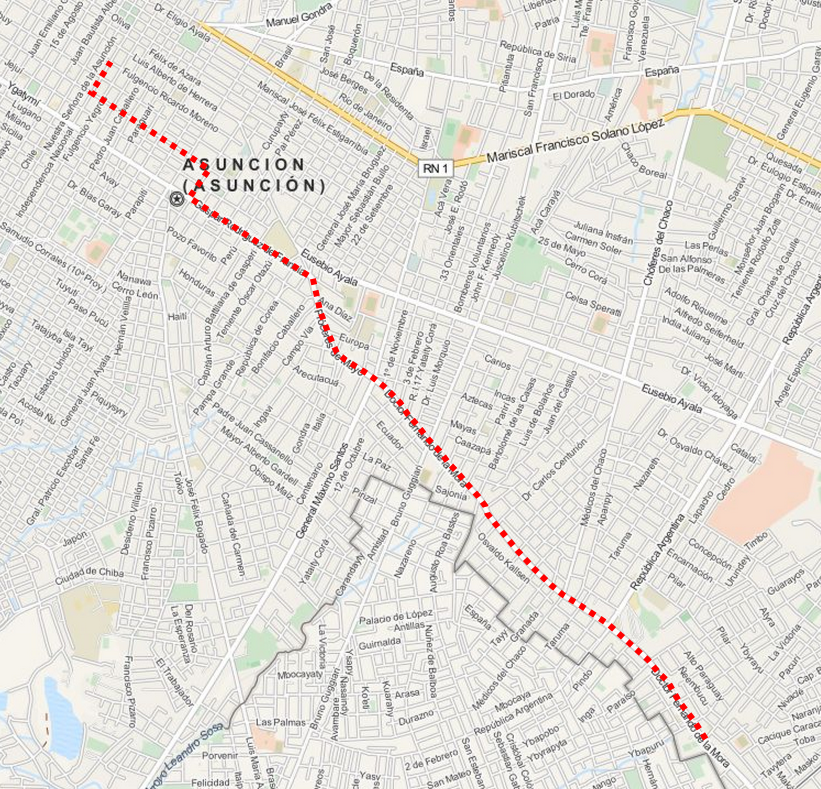
\includegraphics[width=0.35\textwidth]{apartados/figuras/trayecto.png}
	\caption{\label{fig:trayecto} Trayecto de pruebas}	
\end{figure}

Para determinar el valor apropiado del intervalo de reconocimiento, tal que se derive en un balance adecuado entre el consumo de batería y la rápida detección de movimiento, se realizaron pruebas empíricas de 30 iteraciones en el trayecto de recorrido ilustrado por la \Cref{fig:trayecto} con diferentes valores, obteniéndose para cada valor el tiempo promedio que tarda en detectarse el movimiento según se muestra en la \Cref{tab:prom_intervalo_reconocimiento}. Como se puede apreciar en los resultados, un intervalo de reconocimiento corto ayuda a iniciar más rápidamente la toma de localizaciones.


\begin{table}[h]
  \centering
	\begin{tabular}{ccccc}
	\toprule
	Intervalo (s) & Recorridos & En bus (min.) & En auto (min.) & Ambos (min.) \\
	\midrule
	15            & 30       & 1.55         & 1.18            & 1.37         \\
	30            & 30       & 1.64         & 1.30            & 1.47         \\
	45            & 30       & 2.59         & 2.05            & 2.32         \\
	60            & 30       & 4.37         & 2.75            & 3.66         \\
	\bottomrule
	\end{tabular}
  \caption{Tiempos promedio para inicio de rastreo}
  \label{tab:prom_intervalo_reconocimiento}
\end{table}

En base a las pruebas realizadas el intervalo de reconocimiento seleccionado es de 30 segundos, por ser el intervalo más largo que presenta un buen tiempo de respuesta con relación al consumo de batería producido por el número de veces de activación de los sensores. Debe notarse que el tiempo de detección de movimiento para el valor seleccionado, según las pruebas empíricas, oscila en promedio los 1.47 minutos, tiempo en el cual puede considerarse que los sensores fueron activados al menos en 3 oportunidades.

El reconocimiento de actividad también es utilizado para detener la toma de localizaciones cuando el usuario ya no se encuentra en un vehículo en movimiento. Debe tenerse en cuenta también que durante una trayectoria un vehículo puede detenerse momentáneamente debido a diversas causas, como ser un semáforo en rojo o una parada de bus. En estos casos la toma de localizaciones no debe ser erróneamente detenida porque se producirían cortes en la captura del trayecto, y podrían omitirse algunos segmentos debido a que existe un tiempo de espera en la detección de movimiento para reanudar el rastreo como se vio previamente.

Así, para evitar cortes en el rastreo se introduce un \emph{tiempo de tolerancia} en el reconocimiento de actividad. Cada vez que se detecta el movimiento, se almacena el tiempo de detección y el rastreo no es detenido hasta que haya transcurrido el tiempo de tolerancia a partir de la última vez que se detectó movimiento. Se debe tener en cuenta también que un tiempo de tolerancia alto implica que se tardará más en detener el servicio de localización, lo que puede producir un impacto negativo en el consumo de batería debido a la activación innecesaria de los sensores.

Por otra parte, también es importante tener en cuenta el porcentaje de tiempo que el dispositivo estuvo rastreando al usuario con respecto al tiempo total que duró el viaje y que se denomina \emph{tiempo efectivo de rastreo}. Los valores de tiempo de tolerancia e intervalo de reconocimiento en conjunto influyen en el tiempo efectivo de rastreo por lo que deben ser escogidos apropiadamente.

En base al intervalo de reconocimiento de actividad seleccionado previamente, en la \Cref{tab:prom_tiempo_efectivo_rastreo} se muestran resultados acerca del tiempo efectivo de rastreo observado para diferentes valores de tiempo de tolerancia considerados. 

\begin{table}[h]
	\centering
	\begin{tabular}{cccc}
		\toprule
		Intervalo (s) & Tolerancia (min.) & En bus (\%) & En auto (\%) \\
		\midrule
		30            & 3                 & 80.34         & 89.16 \\
		30            & 5                 & 85.86         & 91.56 \\
		30            & 7                & 94.44         & 96.11  \\
		30            & 10                & 95.83         & 97.22 \\
		\bottomrule
	\end{tabular}
	\caption{Tiempos efectivos de rastreo}
	\label{tab:prom_tiempo_efectivo_rastreo}
\end{table}

De las pruebas realizadas puede notarse que con una tolerancia de 10 minutos se obtienen coberturas del 95.83\% en bus y del 97.22\% en auto, tomándose dichos valores como apropiados para este trabajo.

\subsection{Verificación de efectividad de MM}

Para realizar el proceso de MM se utilizó el algoritmo ST-Matching como se describe en \cref{implementacion_mm}. Este algoritmo toma como entrada un conjunto de localizaciones capturadas durante una trayectoria seguida por un usuario para determinar el recorrido correspondiente. Así, el intervalo de tiempo con el que se obtienen dichos puntos se denomina \emph{intervalo de muestreo}. Con un valor de intervalo grande se tiene un menor número de muestras y por ende un menor consumo de batería del dispositivo móvil, pero a su vez podría obtenerse una pobre aproximación del camino recorrido. En cambio, con intervalos pequeños se tiene un mayor número de muestras lo cual aumenta la calidad de la aproximación pero implica un elevado consumo de batería. Finalmente, para medir la efectividad del proceso MM debe observarse la cantidad de puntos que son correctamente asignados a calles al estimar el camino real recorrido.

Las pruebas del proceso de MM consistieron en observar su efectividad con diferentes valores de intervalo de muestreo. Los intervalos observados fueron de 30, 60 y 120 segundos, y para cada intervalo se realizaron 30 recorridos en el trayecto indicado en la \Cref{fig:trayecto}. Para cada valor de intervalo de muestreo se consideró el total de puntos recolectados y se comparó con la cantidad de puntos correctamente asignados. Los resultados obtenidos pueden ser apreciados en la \Cref{table:map_matching}. Puede notarse que se tiene una leve diferencia a favor del intervalo de 30 segundos en comparación al intervalo de 60 segundos y una diferencia un poco mayor en comparación al de 120 segundos. En base a estos resultados se decidió utilizar el intervalo de 60 segundos debido a que implica un menor consumo de batería y produce resultados muy cercanos al intervalo de 30 segundos. Es importante destacar que intervalos menores a 30 segundos no fueron considerados debido a que el algoritmo \emph{ST-Matching} está específicamente diseñado para trabajar con muestras de baja frecuencia \cite{lou2009map}.

\begin{table}[h]
	\centering
	\begin{tabular}{cccc}
        \toprule
    	Intervalo (s) & Total de Puntos & Puntos Correctos & Tasa de Acierto (\%)\\
    	\midrule
    	30 & 1227  & 1141 & 93 \\
    	60 & 594 & 541 & 91 \\
		120 & 313 & 275 & 88 \\  
    	\bottomrule
	\end{tabular}
	\caption{Efectividad del MM} 
	\label{table:map_matching}
\end{table}

\subsection{Análisis de Tráfico}

Para realizar el Análisis de Tráfico se distribuyó la aplicación Autotracks a través de \emph{Google Play}\footnote{https://play.google.com/store} y se observaron los resultados obtenidos de usuarios finales durante un periodo de 5 semanas, en el que se registró un mayor uso de la aplicación. Durante este periodo de tiempo un promedio de 212 usuarios utilizaron diariamente la aplicación, recolectándose un total de 123.419 muestras. En la \Cref{fig:cantidad_usuarios} se observa la cantidad de usuarios activos por día durante el periodo de prueba.

\begin{figure}[h]
	\centering
	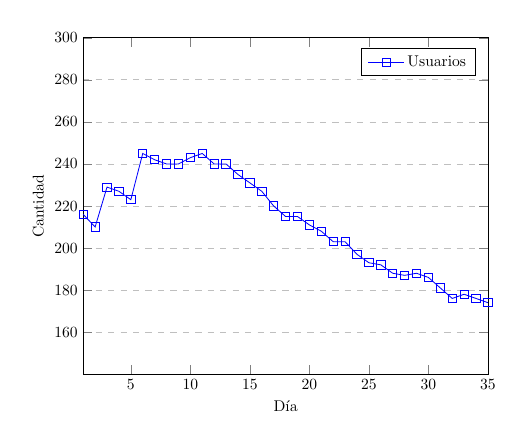
\begin{tikzpicture}[thick,scale=0.75, every node/.style={scale=0.75}]
	\begin{axis}[
	xlabel={Día},
	ylabel={Cantidad},
	xmin=1, xmax=35,
	ymin=140, ymax=300,
	xtick={5,10,15,20,25,30,35},
	ytick={160,180,200,220,240,260,280,300},
	legend pos=north east,
	ymajorgrids=true,
	grid style=dashed,
	]
	
	\addplot[
	color=blue,
	mark=square,
	]
	coordinates {
		(35,174)(34,176)(33,178)(32,176)(31,181)(30,186)(29,188)(28,187)(27,188)(26,192)(25,193)(24,197)(23,203)(22,203)(21,208)(20,211)(19,215)(18,215)(17,220)(16,227)(15,231)(14,235)(13,240)(12,240)(11,245)(10,243)(9,240)(8,240)(7,242)(6,245)(5,223)(4,227)(3,229)(2,210)(1,216)
	};
	\legend{Usuarios}
	
	\end{axis}
	\end{tikzpicture}
	\caption{Cantidad de usuarios activos por día}
	\label{fig:cantidad_usuarios}
\end{figure}

Con el objetivo de caracterizar la actividad de los usuarios a lo largo de una semana, se analizó la distribución de la cantidad de puntos recolectados por día de la semana y por hora del día. Así, en la \Cref{table:localizaciones_por_dia}  puede verse la distribución de muestras por día de la semana, observándose que los lunes son los días en que más localizaciones se recibieron, mientras que en los días domingos se recibió un menor número de localizaciones. Por último, se puede apreciar que en general se recibe una mayor cantidad de localizaciones durante los días entre semana.

\begin{table}[h]
	\centering
	\begin{tabular}{ccc}
        \toprule
    	Día  & Total de Puntos & Promedio\\
    	\midrule
    	Lunes & 20262 & 4052 \\
    	Martes & 18385 & 3677 \\
    	Miércoles & 19361  & 3872 \\ 
    	Jueves & 17833 & 3567 \\
    	Viernes & 18808 & 3762 \\
    	Sábado & 16834 & 3367 \\
    	Domingo & 11936 & 2387 \\
    	\bottomrule
	\end{tabular}
	\caption{Localizaciones tomadas por día de la semana} 
	\label{table:localizaciones_por_dia}
\end{table}

En la \Cref{table:localizaciones_por_hora} se puede observar la distribución de las localizaciones durante las horas del día. Por las mañanas, entre las 6 y 9 horas la mayor cantidad de localizaciones son recibidas y por la tarde entre las 17 y 19 horas. Durante los días entre semana que son normalmente laborales, se hace más notoria esta diferencia. Mientras que durante los fines de semana la horas con mayor cantidad de localizaciones se encuentran hacia el mediodía.

\begin{table}[!h]
	\centering
	\begin{tabular}{cccc}
        \toprule
    	Hora  & Total & Entre semana & Fin de semana\\
    	\midrule
    	00 & 1947 & 1293 & 654 \\
    	01 & 1061 & 424 & 637 \\
    	02 & 1018 & 414 & 604 \\ 
    	03 & 834 & 368 & 466\\
    	04 & 821 & 424 & 397\\
    	05 & 917 & 621 & 296\\
    	06 & 5236 & 4824 & 412 \\
    	07 & 7931 & 7117 & 814\\
    	08 & 9518 & 8586 & 932\\
    	09 & 7326 & 5900 & 1426\\ 
    	10 & 4710 & 3353 & 1357\\
    	11 & 4904 & 3307 & 1597\\
    	12 & 6727 & 4489 & 2238\\
    	13 & 5636 & 3925 & 1711\\
    	14 & 5190 & 3546 & 1644\\
    	15 & 6128 & 4498 & 1630\\
    	16 & 5868 & 4418 & 1450\\ 
    	17 & 6744 & 5287 & 1457\\
    	18 & 10892 & 9204 & 1688\\
    	19 & 9639 & 8018 & 1621\\
    	20 & 7506 & 5815 & 1691\\
    	21 & 6435 & 4525 & 1910\\
    	22 & 4163 & 2933 & 1230 \\
    	23 & 2214 & 1360 & 854\\
    	\bottomrule
	\end{tabular}
	\caption{Localizaciones tomadas por hora del día} 
	\label{table:localizaciones_por_hora}
\end{table}

\begin{table}[h]
	\centering
	\begin{tabular}{cccc}
        \toprule
    	Hora  & Total(km/h) & Entre semana(km/h) & Fines de semana(km/h)\\
    	\midrule
    	00 & 23.2 & 22.3 & 24.9 \\
    	01 & 27.8 & 24.9 & 29.7 \\
    	02 & 30.8 & 33.1 & 29.2 \\ 
    	03 & 31.9 & 36.8 & 28.1\\
    	04 & 38.2 & 47.3 & 31.2\\
    	05 & 33.3 & 29.9 & 40.4\\
    	06 & 17.7 & 16.8 & 28.5\\
    	07 & 19.5 & 18.9 & 24.8\\
    	08 & 18.1 & 16.9 & 28.8\\
    	09 & 19.5 & 17.6 & 27.4\\ 
    	10 & 24.3 & 19.1 & 24.5\\
    	11 & 21.2 & 20.3 & 22.9\\
    	12 & 19 & 17.8 & 21.4\\
    	13 & 19.2 & 18.5 & 20.7\\
    	14 & 23.6 & 20.9 & 29.4\\
    	15 & 22.1 & 20.1 & 27.7\\
    	16 & 20.8 & 19.4 & 24.9\\ 
    	17 & 20.2 & 18.6 & 26,2\\
    	18 & 16.8 & 15.9 & 21.7\\
    	19 & 17.7 & 16.8 & 22.1\\
    	20 & 18.4 & 18.5 & 18.1\\
    	21 & 18.8 & 18.8 & 18.8\\
    	22 & 21.5 & 22.7 & 18.8\\
    	23 & 21.8 & 22.7 & 20.4\\
    	\bottomrule
	\end{tabular}
	\caption{Promedio de velocidad por hora del día} 
	\label{table:velocidad_por_hora}
\end{table}

Finalmente, para caracterizar el flujo de tráfico se escogió como medida la velocidad promedio de desplazamiento de los vehículos, siendo valores mayores de esta mejores y peores los valores bajos. Así, en la \Cref{table:velocidad_por_hora} y la \Cref{fig:promedio_velocidad} se presentan el promedio de velocidad por hora del día y se aprecia que por las mañanas el promedio más bajo de velocidad ocurre entre las 6 y las 9 horas, mientras que por las tardes esto sucede de 18 a 21 horas. También se observa una disminución en la velocidad promedio durante el mediodía. 

En la \Cref{fig:promedio_velocidad_es_fs} se realiza una comparación de modo a contrastar la diferencia que existe en los promedios de velocidad los días entre semana y los fines de semana. Durante los días entre semana se observa un promedio menor de velocidad a partir de las 5 horas hasta las 19 horas. Mientras que los fines de semana se observan dos periodos con bajos valores de velocidad promedio, siendo uno entre las 11 y 13 horas, y otro entre las 20 y 23 horas.

\begin{figure}[h]
\centering
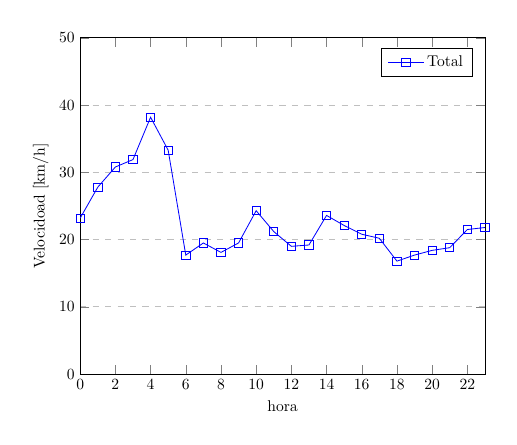
\begin{tikzpicture}[thick,scale=0.75, every node/.style={scale=0.75}]
\begin{axis}[
    xlabel={hora},
    ylabel={Velocidoad [km/h]},
    xmin=0, xmax=23,
    ymin=0, ymax=50,
    xtick={0,2,4,6,8,10,12,14,16,18,20,22},
    ytick={0,10,20,30,40,50},
    legend pos=north east,
    ymajorgrids=true,
    grid style=dashed,
]
 
\addplot[
    color=blue,
    mark=square,
    ]
    coordinates {
    (0,23.2)(1,27.8)(2,30.8)(3,31.9)(4,38.2)(5,33.3)(6,17.7)(7,19.5)(8,18.1)(9,19.5)(10,24.3)(11,21.2)(12,19)(13,19.2)(14,23.6)(15,22.1)(16,20.8)(17,20.2)(18,16.8)(19,17.7)(20,18.4)(21,18.8)(22,21.5)(23,21.8)
    };
    \legend{Total}
 
\end{axis}
\end{tikzpicture}
\caption{Promedio de velocidad por hora del día}
\label{fig:promedio_velocidad}
\end{figure}

\begin{figure}[h]
\centering
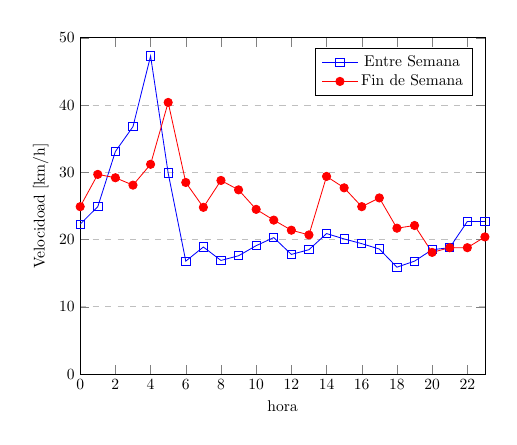
\begin{tikzpicture}[thick,scale=0.75, every node/.style={scale=0.75}]
\begin{axis}[
    xlabel={hora},
    ylabel={Velocidoad [km/h]},
    xmin=0, xmax=23,
    ymin=0, ymax=50,
    xtick={0,2,4,6,8,10,12,14,16,18,20,22},
    ytick={0,10,20,30,40,50},
    legend pos=north east,
    ymajorgrids=true,
    grid style=dashed,
]
 
\addplot[
    color=blue,
    mark=square,
    ]
    coordinates {
    (0,22.3)(1,24.9)(2,33.1)(3,36.8)(4,47.3)(5,29.9)(6,16.8)(7,18.9)(8,16.9)(9,17.6)(10,19.1)(11,20.3)(12,17.8)(13,18.5)(14,20.9)(15,20.1)(16,19.4)(17,18.6)(18,15.9)(19,16.8)(20,18.5)(21,18.8)(22,22.7)(23,22.7)
    };
    \addlegendentry{Entre Semana}

\addplot[
    color=red,
    mark=*,
    ]
    coordinates {
    (0,24.9)(1,29.7)(2,29.2)(3,28.1)(4,31.2)(5,40.4)(6,28.5)(7,24.8)(8,28.8)(9,27.4)(10,24.5)(11,22.9)(12,21.4)(13,20.7)(14,29.4)(15,27.7)(16,24.9)(17,26.2)(18,21.7)(19,22.1)(20,18.1)(21,18.8)(22,18.8)(23,20.4)
    };
    \addlegendentry{Fin de Semana}
 
\end{axis}
\end{tikzpicture}
\caption{Comparativa de promedios de velocidad por hora}
\label{fig:promedio_velocidad_es_fs}
\end{figure}

\subsection{Aproximación del Tráfico en Tiempo Real}

Para aproximar el estado del tráfico en tiempo real, se obtiene el promedio de velocidad de todos los puntos que hayan sido asociados a un segmento de calle en particular durante la última hora. De esta forma, es posible presentar información del estado del tráfico en aquellas calles que han sido transitadas recientemente. En contrapartida, para aquellas calles que no cuentan con información reciente, no se presentan una aproximación de su estado. A modo de ilustración, en la \Cref{fig:trafico_en_tr} se muestra el estado del tráfico aproximado en tiempo real para un día entre semana, entre las 9 y 17 horas. Se puede observar cómo el estado de los segmentos de calles va variando a lo largo del día, conforme a los datos recolectados.

\begin{figure*}[!htbp]
	\centering
	\begin{subfigure}[b]{0.25\textwidth}
		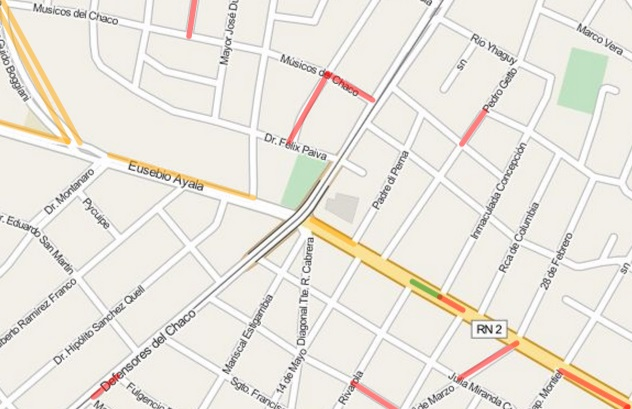
\includegraphics[width=\textwidth]{apartados/figuras/9.jpg}
		\caption{9:00}
	\end{subfigure}
	~~
	\begin{subfigure}[b]{0.25\textwidth}
		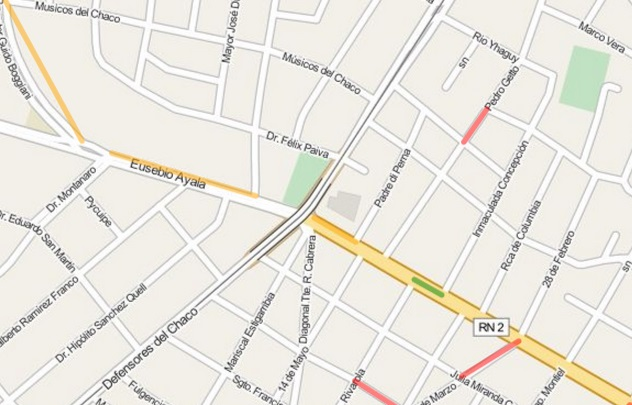
\includegraphics[width=\textwidth]{apartados/figuras/10.jpg}
		\caption{10:00}
	\end{subfigure}
	~~
	\begin{subfigure}[b]{0.25\textwidth}
		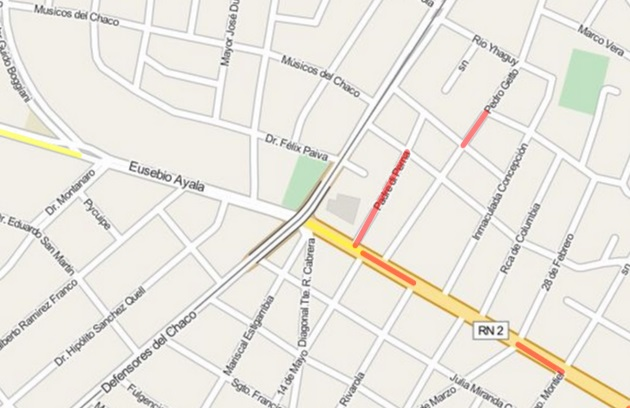
\includegraphics[width=\textwidth]{apartados/figuras/11.jpg}
		\caption{11:00}
	\end{subfigure}
	
	\begin{subfigure}[b]{0.25\textwidth}
		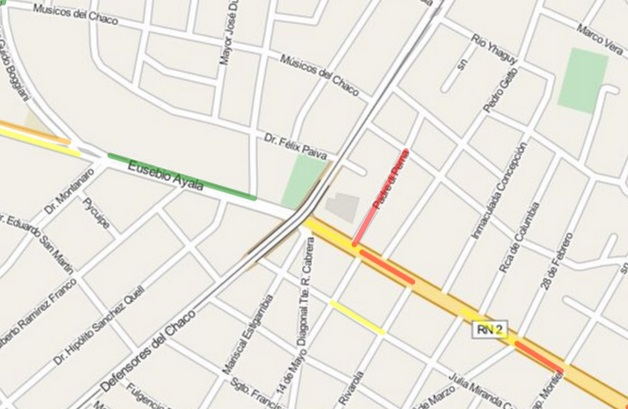
\includegraphics[width=\textwidth]{apartados/figuras/12.jpg}
		\caption{12:00}
	\end{subfigure}
	~~
	\begin{subfigure}[b]{0.25\textwidth}
		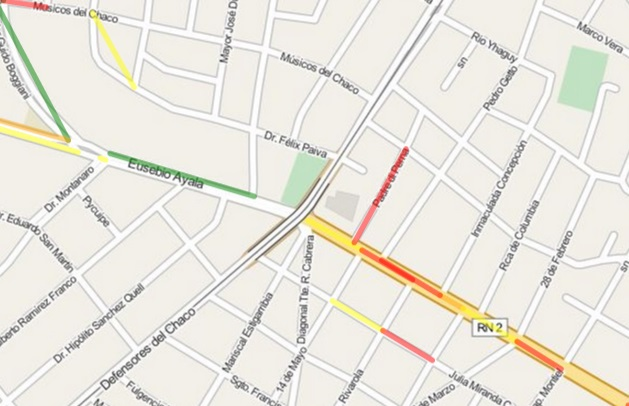
\includegraphics[width=\textwidth]{apartados/figuras/13.jpg}
		\caption{13:00}
	\end{subfigure}
	~~
	\begin{subfigure}[b]{0.25\textwidth}
		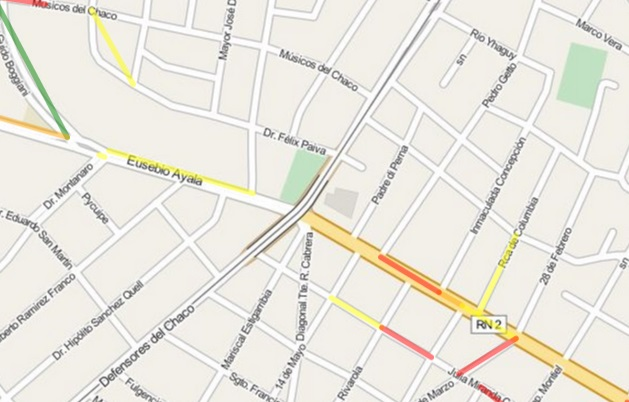
\includegraphics[width=\textwidth]{apartados/figuras/14.jpg}
		\caption{14:00}
	\end{subfigure}
	
	\begin{subfigure}[b]{0.25\textwidth}
		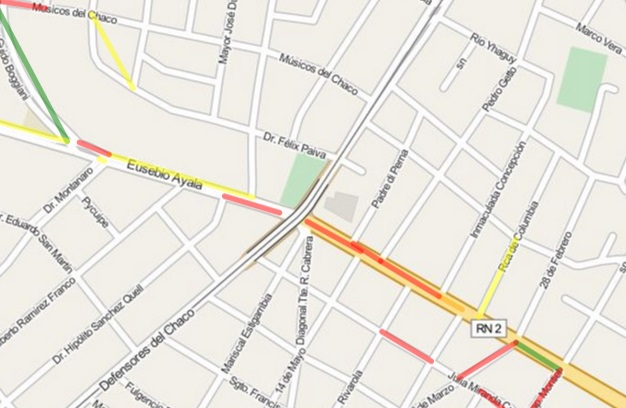
\includegraphics[width=\textwidth]{apartados/figuras/15.jpg}
		\caption{15:00}
	\end{subfigure}
	~~
	\begin{subfigure}[b]{0.25\textwidth}
		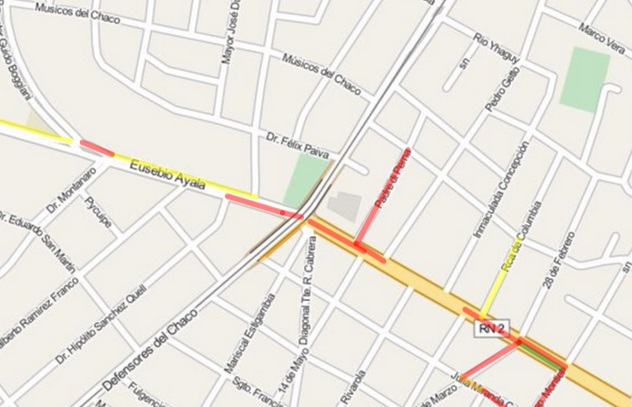
\includegraphics[width=\textwidth]{apartados/figuras/16.jpg}
		\caption{16:00}
	\end{subfigure}
	~~
	\begin{subfigure}[b]{0.25\textwidth}
		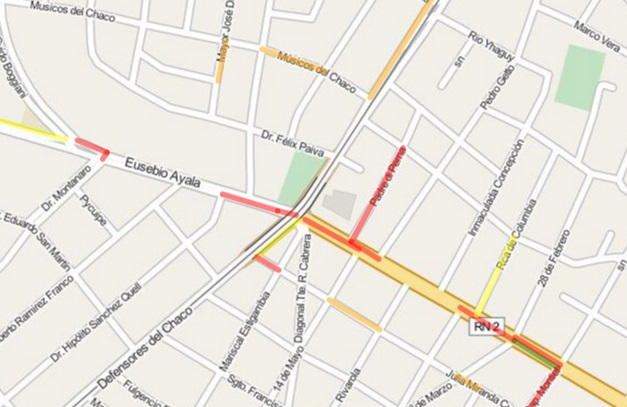
\includegraphics[width=\textwidth]{apartados/figuras/17.jpg}
		\caption{17:00}
	\end{subfigure}
	\caption{Tráfico en un tramo a lo largo del día}
	\label{fig:trafico_en_tr} 
\end{figure*}